\documentclass[tikz, border = 2pt, varwidth]{standalone}

%---------------------------------------------------------------------------%
% PACKAGES                                                                  %
%---------------------------------------------------------------------------%

%----- MATH
%---------------------------------------------------------------------------%
\usepackage{amsmath, amssymb}

%----- FIGURES
%---------------------------------------------------------------------------%
\usepackage{pgfplots}
\usetikzlibrary{patterns}
\pgfplotsset{compat=1.13}

\begin{document}
	
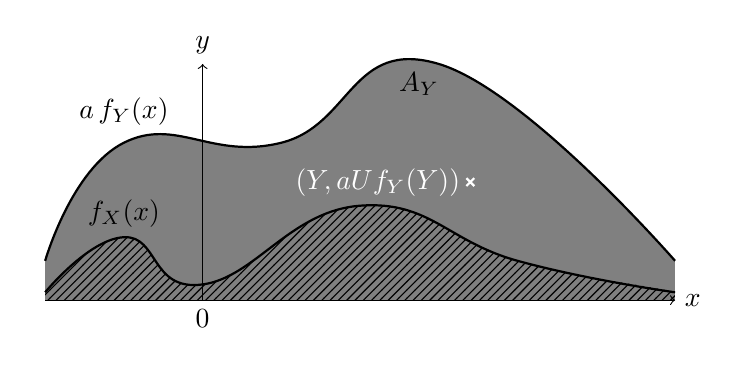
\begin{tikzpicture}
	\fill [fill = black!50] (-2,0) rectangle (6,0.5);
	\fill[thick, fill = black!50, draw = black] plot [smooth,tension=.8] coordinates{(-2,0.5) (-1,2) (1,2) (3,3) (6,0.5)};
	\fill[pattern=north east lines] plot [smooth,tension=.8] coordinates{(-2,0) (-2,0.1) (-1,0.8) (0,0.2) (2,1.2) (4,0.5) (6,0.1) (6,0)};
	\fill[fill = white] (-2.2,-0.1) rectangle (-2,0.1);
	\fill[fill = white] (6,-0.1) rectangle (6.2,0.1);
	\draw[thick, draw = black] plot [smooth,tension=.8] coordinates{(-2,0.1) (-1,0.8) (0,0.2) (2,1.2) (4,0.5) (6,0.1)};
	\draw[->] (-2,0) -- (6,0) node[anchor = west] {$x$};
	\draw[->] (0,0) -- (0,3) node[anchor = south] {$y$};
	\node[anchor = north] at (0,0) {$0$};
	\node at (2.75,2.75) {$A_Y$};
	\draw[mark=x, white, thick] plot coordinates {(3.4,1.5)} node[anchor = east] {\color{white}$(Y,aUf_Y(Y))$};
	\node at (-1,2.4) {$a\,f_Y(x)$};
	\node at (-1,1.1) {$f_X(x)$};
\end{tikzpicture}

\end{document}